\documentclass[letterpaper,12pt]{article}
\usepackage[utf8]{inputenc}
\usepackage[russian]{babel}
\usepackage[left=2cm,right=2cm,top=2cm,bottom=2cm,bindingoffset=0cm]{geometry}
\usepackage{graphicx}
\graphicspath{{images/}}
\usepackage{float}
\usepackage{wrapfig}


\begin{document}
\begin{center}
Описание возможных случаев поведения алгоритма в процессе <<перешагивания>>
ребра
\end{center}
Как входные данные имеем: 
\begin{enumerate}
      \item Контейнер упорядоченных по полярному углу относительно
            прошлой грани точек.
      \item Индексы $i, j$ точек, задающих <<перешагиваемое>> ребро.
      \item Отрезки, концами которых являются данные точки.
      \item Информация о правильности затронутых отрезков.
\end{enumerate}
Не умоляя общности, рассмотрим случаи для ребра расположенного вертикально:
\begin{enumerate}
      \item Точки $p_i, p_j$ являются точками одного отрезка. Так как
            варианты с <<перешагиванием>> отрезка исключены из рассмотрения,
            вожможен только изображенный ниже случай и его зеркальная версия.
            \par
            Действие -- точки $p_i, p_j$ меняются местами в массиве, 
            <<правильность>> отрезка остается неизменной.
            \begin{figure}[h]
            \centering
            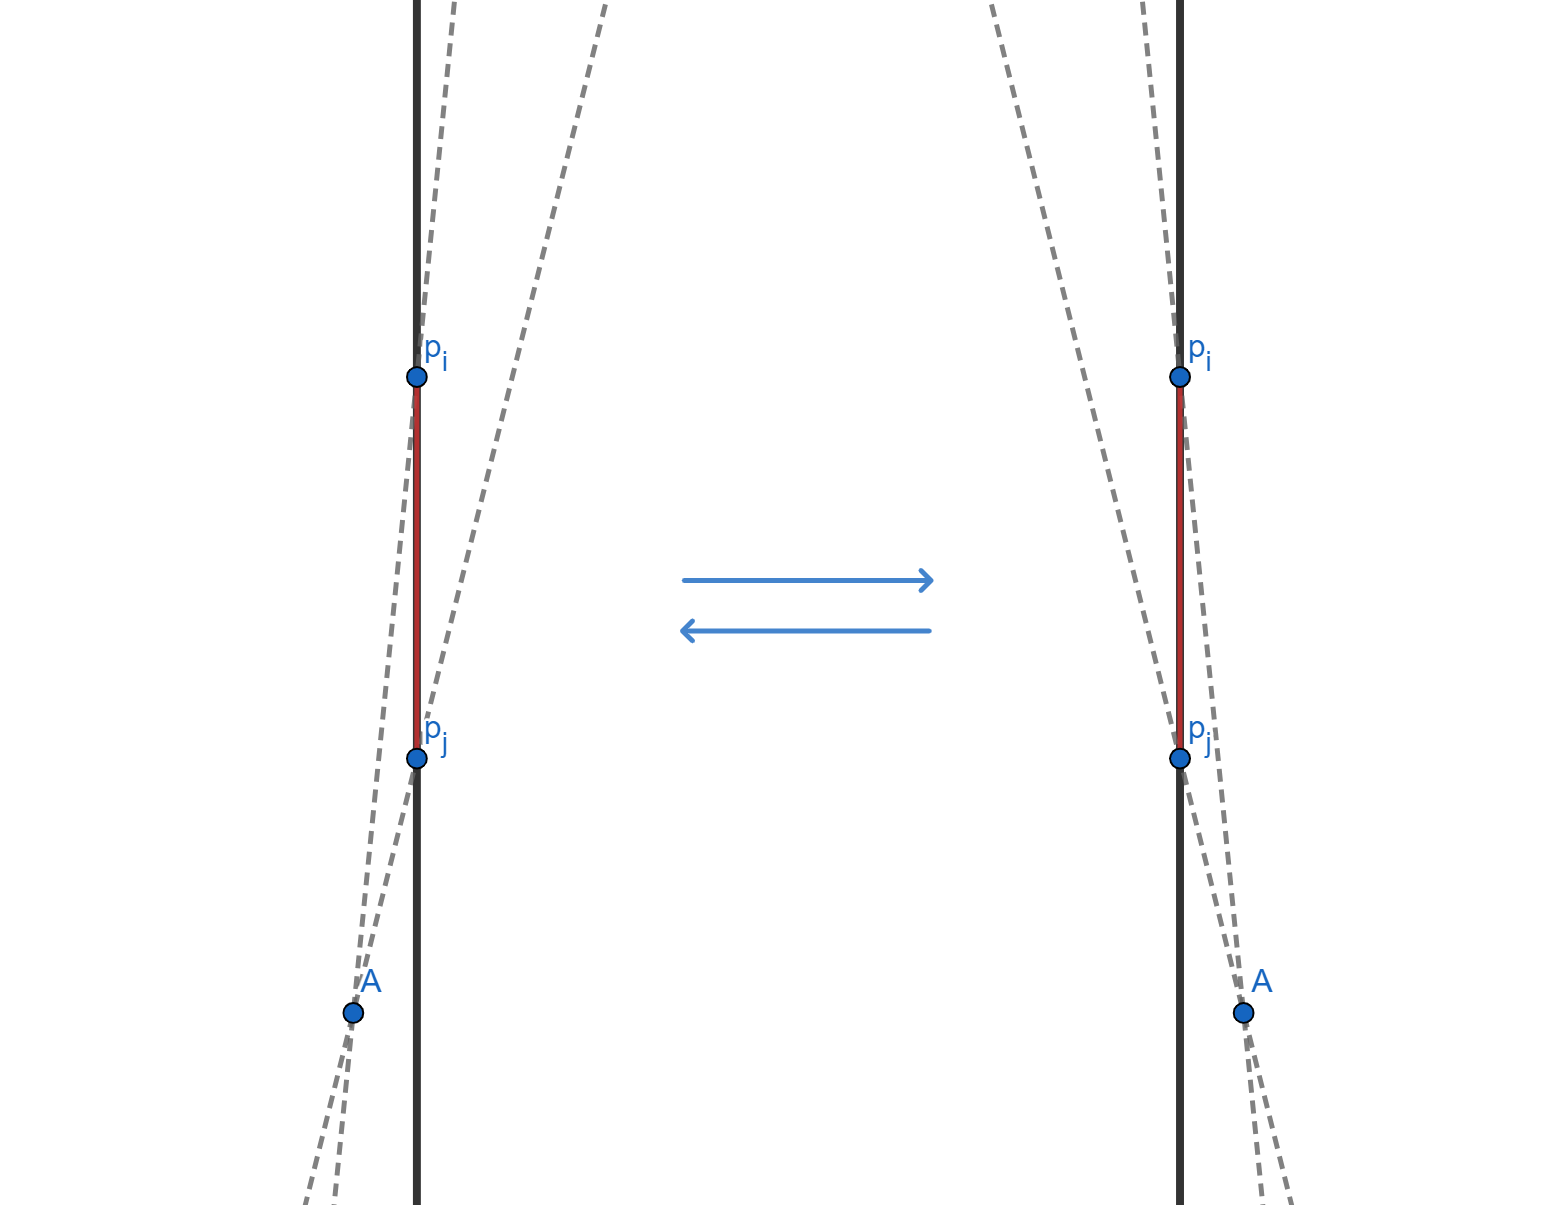
\includegraphics[width=.5\linewidth]{one_segment.png}
            \end{figure}
      \item Точки $p_i, p_j$ лежат на прямой с одной стороны относительно
            <<Перешагиваемого>> ребра. Возможны варианты, изображенные ниже,
            а также зеркальные к ним.
            \par
            Действие -- точки $p_i, p_j$ меняются местами в массиве.
            <<Правильность>> обоих отрезков необходимо пересчитать честно.
            \begin{figure}[H]
            \centering
            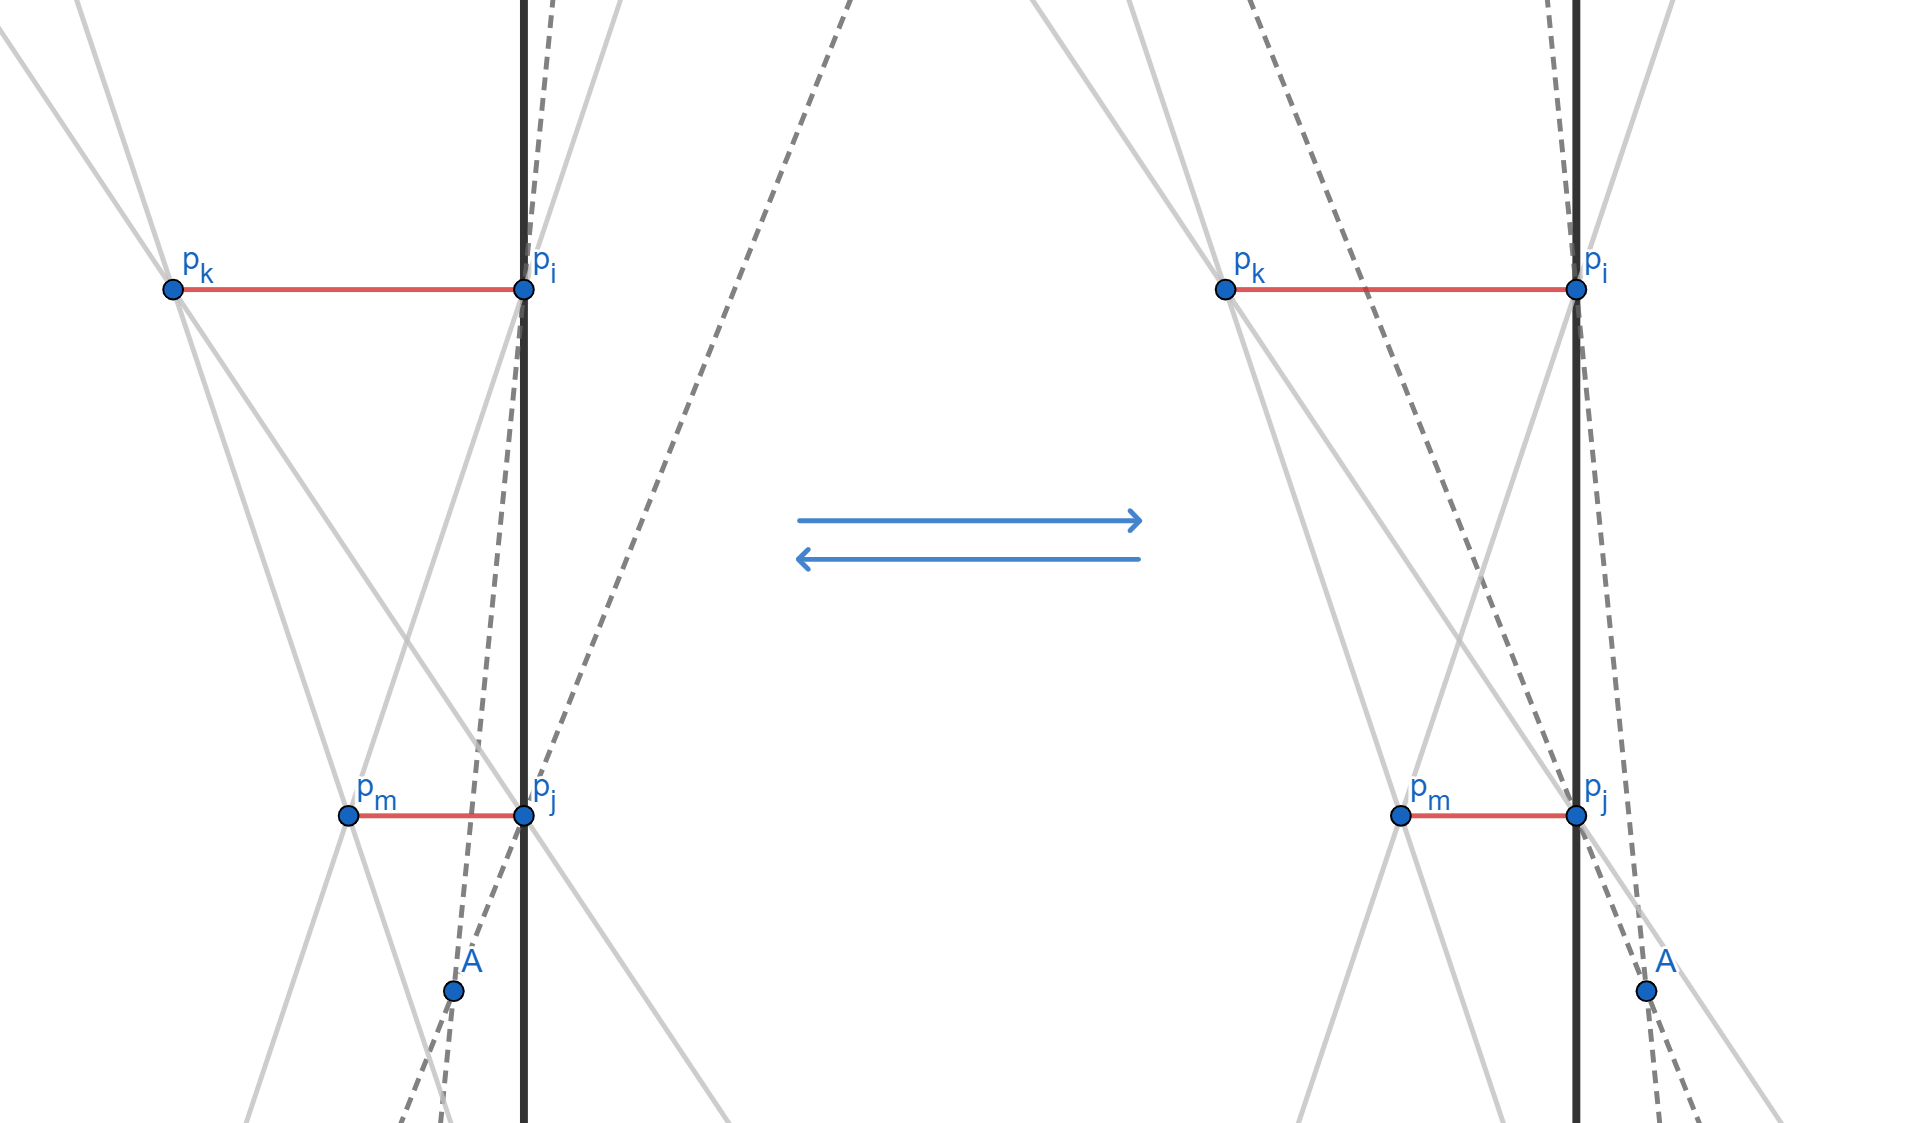
\includegraphics[width=.6\linewidth]{one_side_1.png}
            \end{figure}
            \begin{figure}[H]
            \centering
            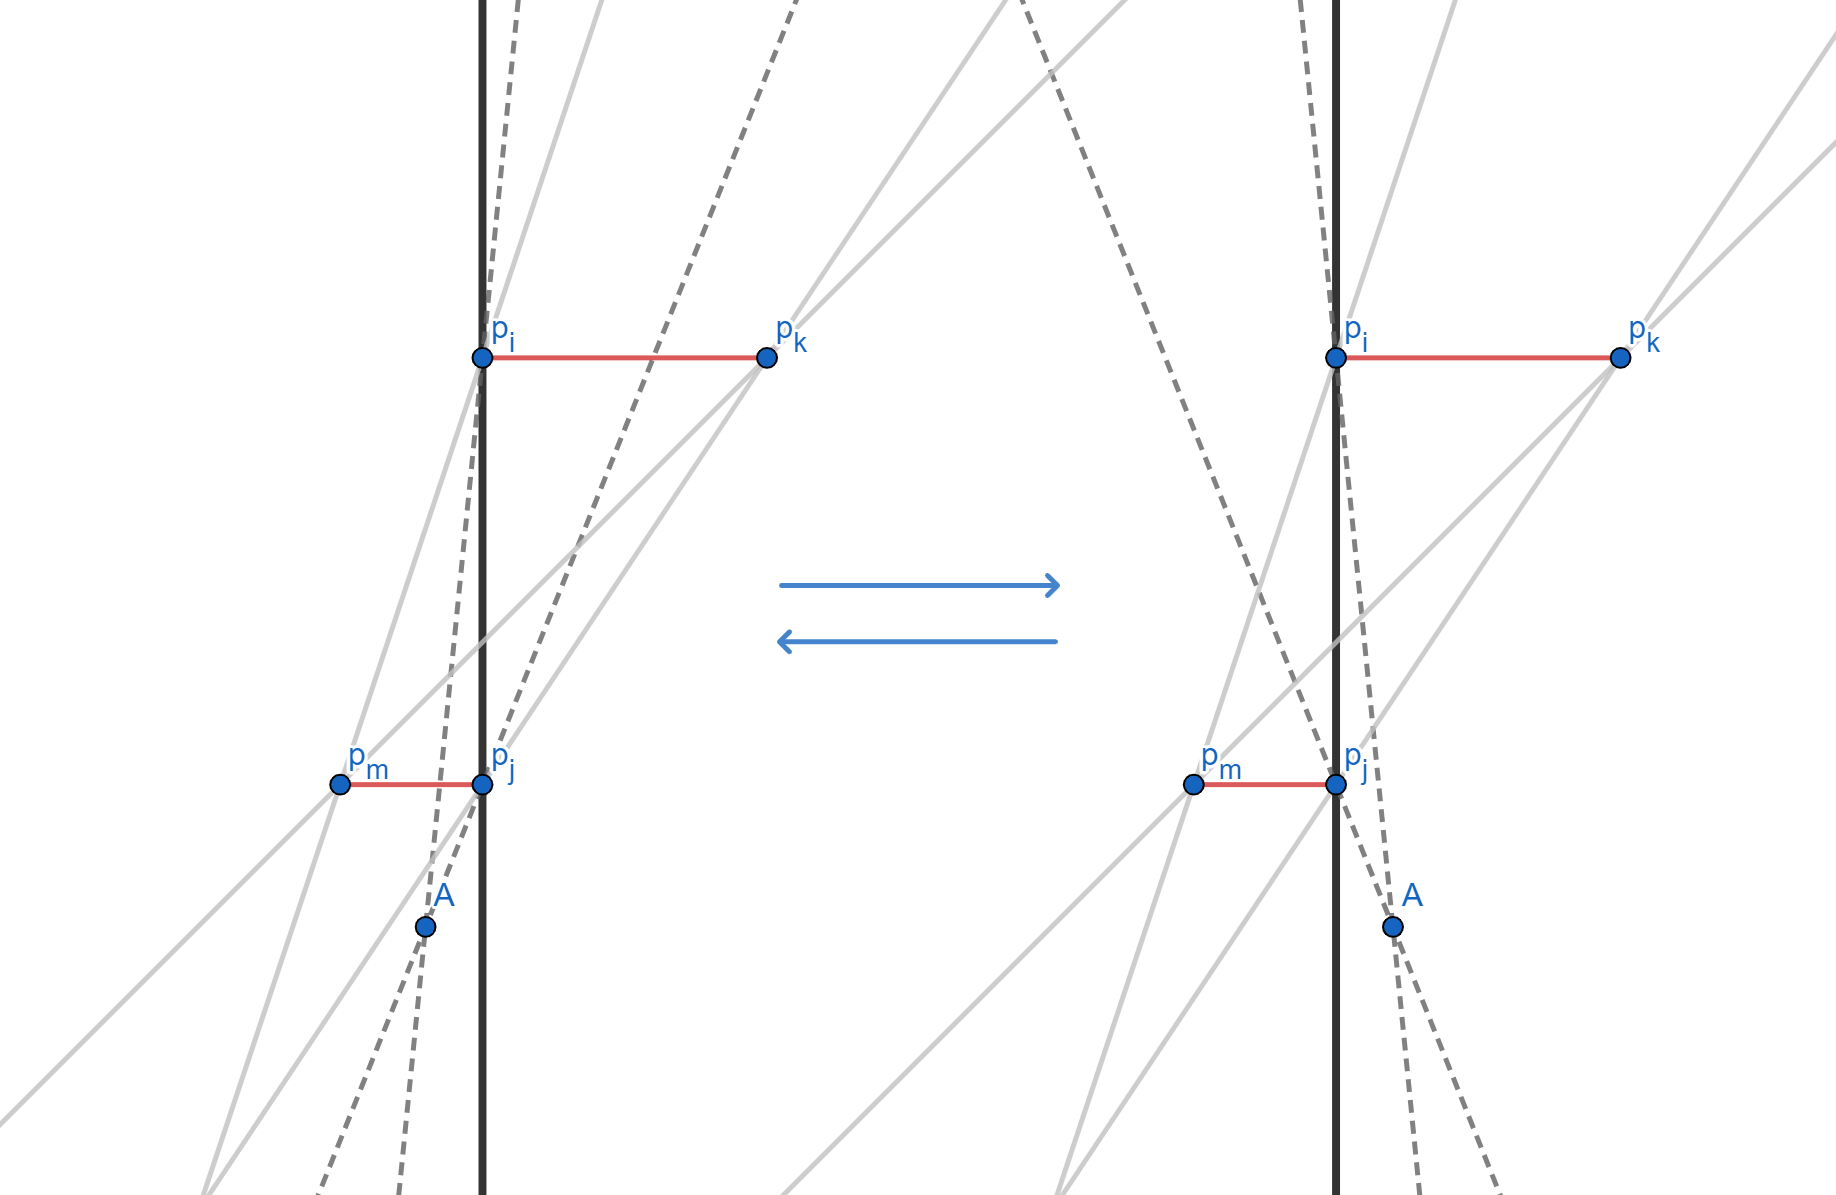
\includegraphics[width=.6\linewidth]{one_side_2.png}
            \end{figure}
      \item Точки $p_i, p_j$ лежат на прямой по разные стороны 
            относительно <<Перешагиваемого>> ребра. Возможны варианты, 
            изображенные ниже, а также зеркальные к ним.
            \par
            Действие -- без изменений.
            \begin{figure}[H]
            \centering
            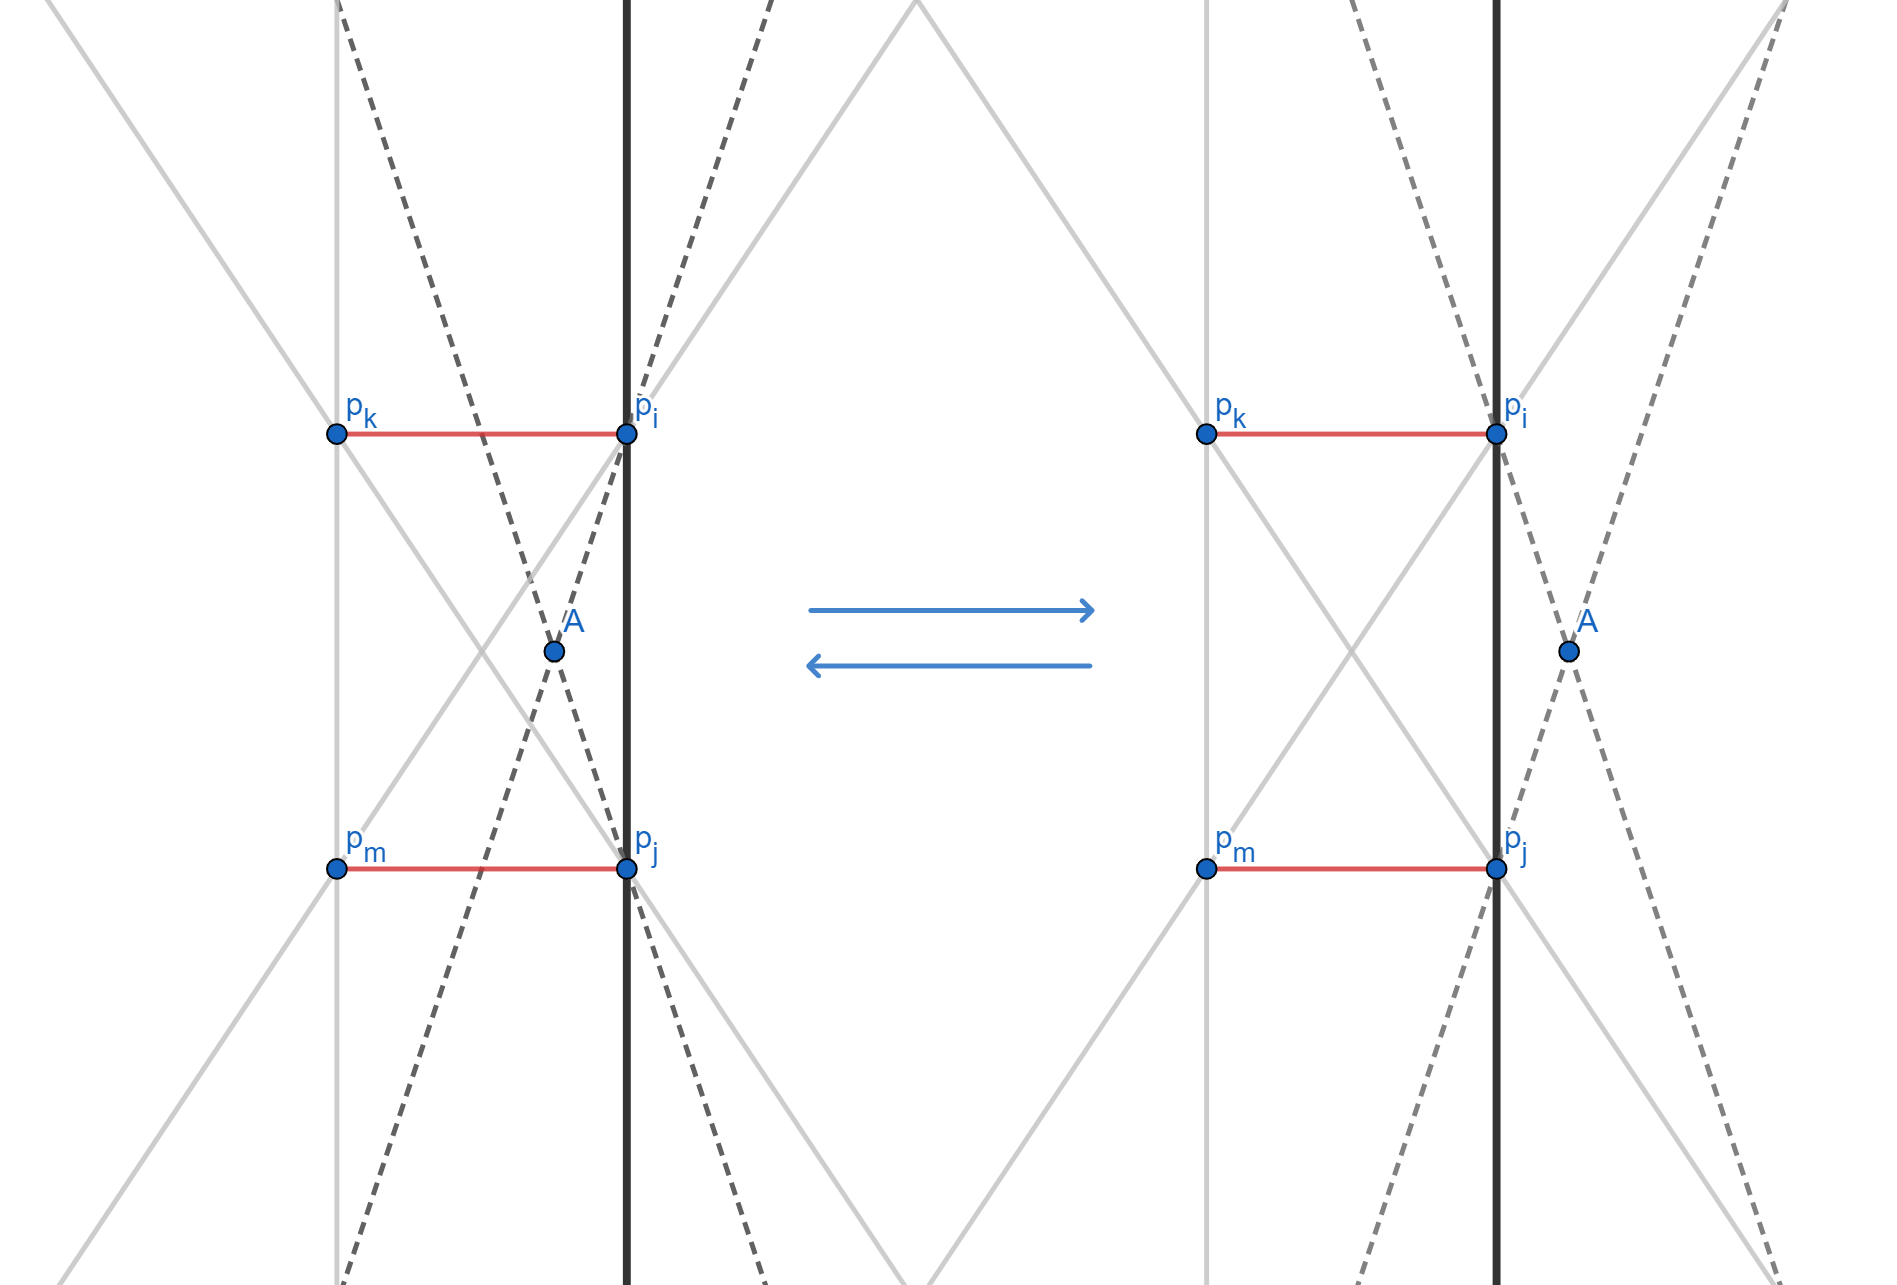
\includegraphics[width=.6\linewidth]{between_1.png}
            \end{figure}
            \begin{figure}[H]
            \centering
            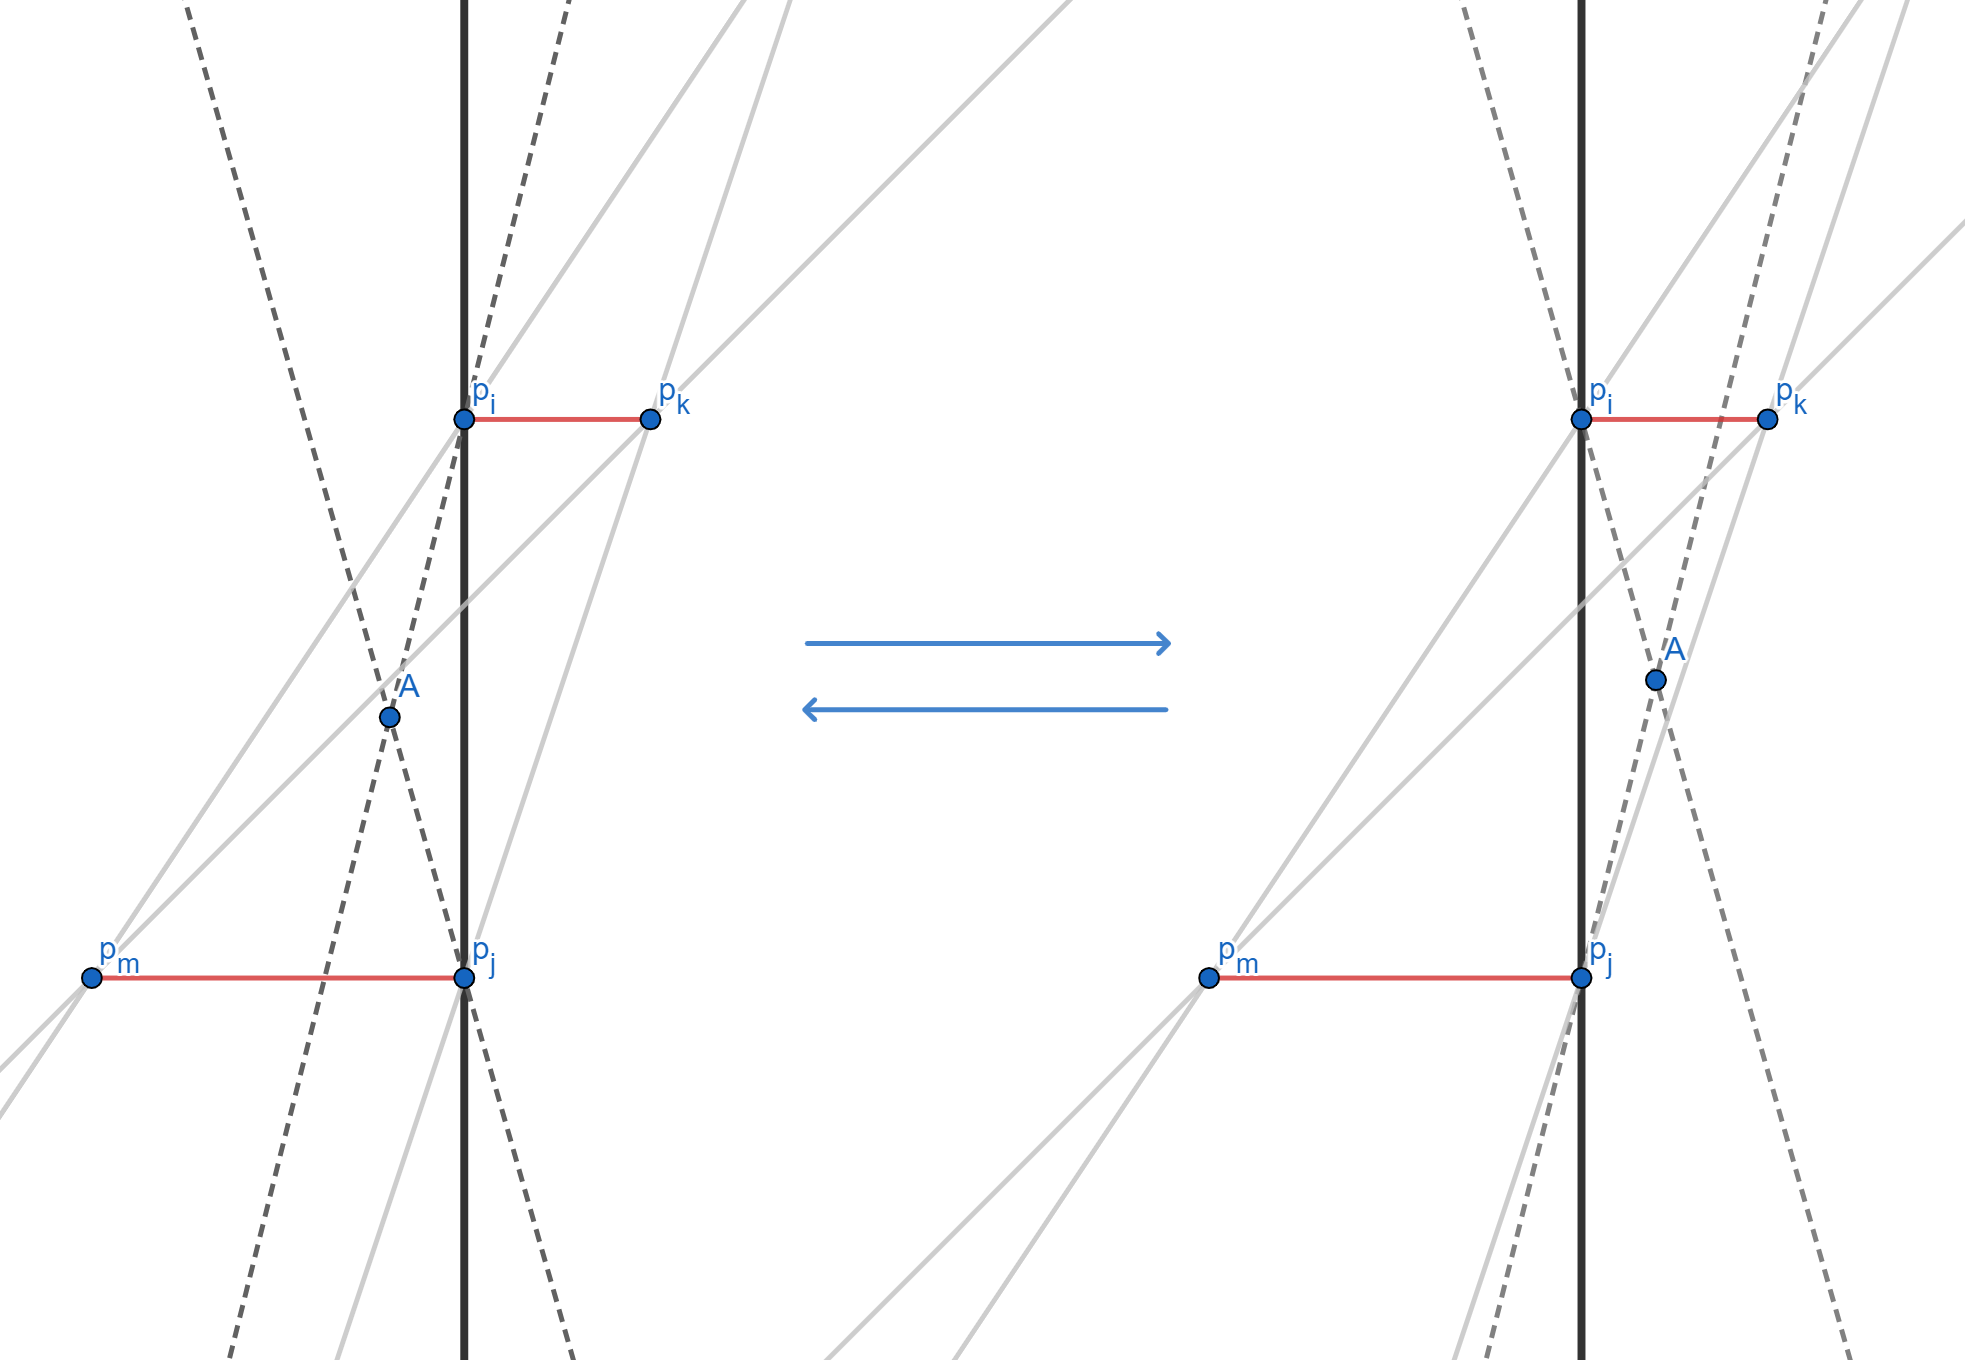
\includegraphics[width=.6\linewidth]{between_2.png}
            \end{figure}
\end{enumerate}
\end{document}